\documentclass[12pt,a4paper]{article}

\usepackage[latin1]{inputenc}
\usepackage{amsmath}
\usepackage{amsfonts}
\usepackage{amssymb}
\usepackage{amsthm}
\usepackage{enumitem}
\usepackage[english]{babel}
\usepackage{fancyhdr}
\usepackage{lipsum}
\usepackage{chngpage}
\usepackage{geometry}
\usepackage{mathtools}
\usepackage{tabularx}
\usepackage{verbatim}
\usepackage{tikz}
\usepackage[ruled,vlined]{algorithm2e}
\geometry{legalpaper, portrait, margin=1in}
 
\pagestyle{fancy}
\fancyhf{}
\rhead{\thepage}
\lhead{A Path 3-List-Coloring Algorithm for Plane Graphs}
\rfoot{}

\newcommand{\overbar}[1]{\mkern 1.5mu\overline{\mkern-1.5mu#1\mkern-1.5mu}\mkern 1.5mu}

\begin{document}

\title{A Path 3-List Coloring Algorithm for Plane Graphs}
\date{March 28, 2016}
\author{Aven Bross}

\maketitle

\section*{Abstract}

We present an algorithm to path $3$-list-color plane graphs based on the work by Skrekovski [2]
and Hartman [1]. Furthermore, we provide implementation details and an efficient implementation of the
algorithm in the Boost Graph Library.

\section{Introduction}

\noindent All graphs discussed are assumed to be simple, undirected, and plane embeded. For plane embeddings we assume
the edges around each vertex are arranged in clockwise order. For a graph $G$, let $V(G)$ denote its vertex set
and $E(G)$ denote the edge set.\\

\noindent Using notation from [1], for $v\in V(G)$ we will denote the \emph{neighborhood} of $v$ in $G$ as
$N_G(x)=\{u\in V(G)\mid uv\in E(G)\}$. For $u,w\in N_G(v)$ we will use $[u,w]_v$ and $(u,w)_v$ to denote the ordered list of vertices between $u$
and $w$ in $N_G(v)$ in clockwise embedded order, inclusive and exclusive respectively. We will use $[u,w]'_v$ and $(u,w)'_v$ for the
equivalent counterclockwise listings. Furthermore, if $C$ is the outer face of a weakly triangulated $2$-connected
graph then for $u,v\in C$ let $C[u,v]$ denote the set of
vertices along the outer face in clockwise order between $u$ and $v$ inclusive. \\

\noindent A \emph{path} is a graph $P$ with $V(P)=\{v_1,v_2,v_3,\ldots,v_n\}$ and $E(P)=\{v_1v_2,v_2v_3,\ldots,v_{n-1}v_n\}$.
It is common to refer to $P$ as a $v_1v_n$-path. A graph $G$ is connected if for every pair of vertices
$u,v\in G$, there exists a $uv$-path subgraph of $G$. All graphs discussed in this project are connected. For a vertex
$v\in G$, if removing $v$ disconnects $G$, then $v$ is known as a cutvertex. A graph is considered
\emph{biconnected} if it contains no cutvertices.\\

\noindent A \emph{coloring} of a graph $G$ assigns a color to each vertex. If $L(v)$ assigns
a list of $k$ colors to each vertex $v\in V(G)$, a \emph{$k$-list-coloring} colors $G$ such
that each $v\in V(G)$ is colored from $L(v)$. A \emph{path $k$-list-coloring} is a $k$-list-coloring such that
each color class induces a disjoint union of paths.

\section{Vertex Removal}

In this section we present two theorems describing the effects of vertex removal on weakly triangulated plane
graphs. These will be necessary in later
sections to remove already colored paths from our graph. First, we consider removing a vertex
from the outer face that has only two neighbors in the outer face (i.e. no chords).\\

\begin{adjustwidth}{2em}{2em}
\noindent \textbf{Theorem 1.} Let $G$ be a weakly triangulated biconnected plane graph with $|V(G)|\ge 4$ and
outer face
$C=c_0c_1\ldots c_{n-1}$ in clockwise embedded order. Then $N_C(c_0)=\{c_{1},c_{n-1}\}$ if and only if
$G_0=G-c_1$ is a weakly triangulated plane graph with $|V(G_0)|\ge 3$ and outer face
$C_0=c_1\ldots c_{n-1}(c_{1},c_{n-1})'_{c_0}$.

\begin{proof}
First notice that $G_0$ is clearly weakly triangulated since $G$ was weakly triangulated and we removed a
vertex from the outer face.
Let $u,v\in G_0$. If $u,v\in C_0$ then there are clearly two edge disjoint $uv$-paths. If $u\in C_0$ and $v\not\in C_0$,
there are two edge disjoint paths $v$ to $C_0$, thus two edge disjoint $uv$-paths. Finally,
if $u,v\not\in C_0$ then we may find two edge disjoint paths from $u$ to $C_0$ and two disjoint paths $v$ to $C_0$ and
join each pair using the outer cycle.
Clearly in each case we have two edge disjoint $uv$-paths and $G_0$ is biconnected.
\end{proof}
\end{adjustwidth}

\begin{adjustwidth}{2em}{2em}
\begin{center}
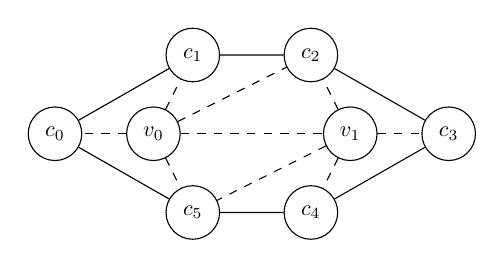
\begin{tikzpicture}[scale=1, every node/.style={circle, draw, minimum size=8.5mm, scale=.8}]
  \node (c0) at (-2.5cm,0cm) {$c_0$};
  \node (c1) at (-0.75cm,1cm) {$c_1$};
  \node (c2) at (0.75cm,1cm) {$c_2$};
  \node (c3) at (2.5cm,0cm) {$c_3$};
  \node (c5) at (-0.75cm,-1cm) {$c_5$};
  \node (c4) at (0.75cm,-1cm) {$c_4$};
  \node (v1) at (1.25cm,0cm) {$v_1$};
  \node (v0) at (-1.25cm,0cm) {$v_0$};
  
  \draw (c0) -- (c1) -- (c2) -- (c3) -- (c4) -- (c5) -- (c0);
  \draw (v0)-- (c0) [dashed]; \draw (v0)-- (c1) [dashed]; \draw (v0)-- (c2) [dashed]; \draw (v0)-- (v1) [dashed];
  \draw (v0)-- (c5) [dashed];  \draw (v1)-- (c2) [dashed]; \draw (v1)-- (c3) [dashed]; \draw (v1)-- (c4) [dashed]; \draw (v1)-- (c5) [dashed]; 
\end{tikzpicture}
$\qquad$
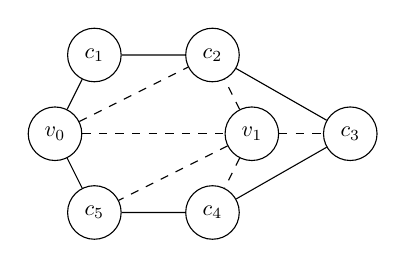
\begin{tikzpicture}[scale=1, every node/.style={circle, draw, minimum size=8.5mm, scale=.8}]
  \node (c1) at (-0.75cm,1cm) {$c_1$};
  \node (c2) at (0.75cm,1cm) {$c_2$};
  \node (c3) at (2.5cm,0cm) {$c_3$};
  \node (c5) at (-0.75cm,-1cm) {$c_5$};
  \node (c4) at (0.75cm,-1cm) {$c_4$};
  \node (v1) at (1.25cm,0cm) {$v_1$};
  \node (v0) at (-1.25cm,0cm) {$v_0$};
  
  \draw (c1) -- (c2) -- (c3) -- (c4) -- (c5); \draw (v0)-- (c1); \draw (v0)-- (c2) [dashed]; \draw (v0)-- (v1) [dashed];
  \draw (v0)-- (c5);  \draw (v1)-- (c2) [dashed]; \draw (v1)-- (c3) [dashed]; \draw (v1)-- (c4) [dashed]; \draw (v1)-- (c5) [dashed]; 
\end{tikzpicture}
\hfill\\
\hfill\\
\footnotesize{Removing $c_0$ with Theorem 1.}
\end{center}
\end{adjustwidth}
\hfill

\noindent Using the previous statement we produce a stronger statement describing the result of removing any outer face
vertex from a weakly triangulated graph. A \emph{block} of a graph $G$ is a maxmimal subgraph $H$ of $G$ such
that $H$ is biconnected or a complete graph on $1$ or $2$ vertices.\\

\begin{adjustwidth}{2em}{2em}
\noindent \textbf{Theorem 2.} Let $G$ be a weakly triangulated biconnected plane graph with $|V(G)|\ge 3$ and outer face
$C=c_0c_1\ldots c_{n-1}$ in clockwise embedded order. Then $G-c_0$ may be divided up into one or more blocks
$G_0,\ldots,G_k$ such that $G-c_0=G_0\cup G_1\cup\ldots\cup G_k$, each $G_i$ has $|V(G_i)|\ge2$, and each
$G_i$ is weakly triangulated if $|V(G_i)|\ge3$. Furthermore, each $G_i$ has at most two cutvertices.

\begin{proof}
Notice if $|V(G)|=3$, then $G-c_0$ is a complete graph on $2$ vertices. Suppose $|V(G)|\ge4$. If 
$N_C(c_0)=\{c_1,c_n\}$ then Theorem 1 applies. Otherwise, there exists $c_i\in N_C(c_0)$ distinct from $c_1$ and
$c_n$. Let us then recurse on the subgraph bounded by $c_0c_1\ldots c_i$ and the subgraph bounded by
$c_ic_{i+1}\ldots c_nc_0$. Note that after removing $c_0$ each subgraph will only have the
cutvertex $c_i$ in common.
\end{proof}
\end{adjustwidth}

\begin{adjustwidth}{2em}{2em}
\begin{center}
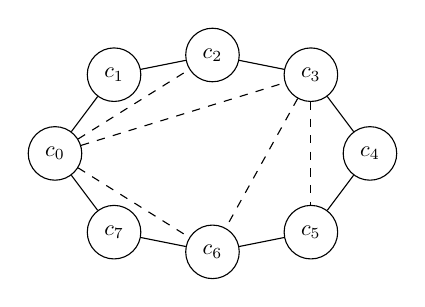
\begin{tikzpicture}[scale=1, every node/.style={circle, draw, minimum size=8.5mm, scale=.8}]
  \node (c0) at (-2cm,0cm) {$c_0$};
  \node (c1) at (-1.25cm,1cm) {$c_1$};
  \node (c2) at (0cm,1.25cm) {$c_2$};
  \node (c3) at (1.25cm,1cm) {$c_3$};
  \node (c4) at (2cm,0cm) {$c_4$};
  \node (c5) at (1.25cm,-1cm) {$c_5$};
  \node (c6) at (0cm,-1.25cm) {$c_6$};
  \node (c7) at (-1.25cm,-1cm) {$c_7$};
  
  \draw (c0) -- (c1) -- (c2) -- (c3) -- (c4) -- (c5) -- (c6) -- (c7) -- (c0);
  \draw (c0)-- (c2) [dashed]; \draw (c0)-- (c3) [dashed]; \draw (c0)-- (c6) [dashed];
  \draw (c3)-- (c6) [dashed];\draw (c3)-- (c5) [dashed];
\end{tikzpicture}
$\qquad$
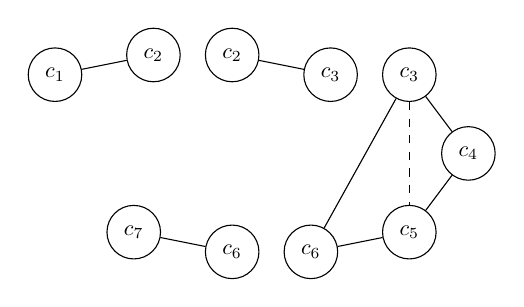
\begin{tikzpicture}[scale=1, every node/.style={circle, draw, minimum size=8.5mm, scale=.8}]
  \node (0c1) at (-1.25cm,1cm) {$c_1$};
  \node (0c2) at (0cm,1.25cm) {$c_2$};
  
  \node (1c2) at (1cm,1.25cm) {$c_2$};
  \node (1c3) at (2.25cm,1cm) {$c_3$};
  
  \node (c3) at (3.25cm,1cm) {$c_3$};
  \node (c4) at (4cm,0cm) {$c_4$};
  \node (c5) at (3.25cm,-1cm) {$c_5$};
  \node (c6) at (2cm,-1.25cm) {$c_6$};
  
  \node (2c6) at (1cm,-1.25cm) {$c_6$};
  \node (2c7) at (-0.25cm,-1cm) {$c_7$};
  
  \draw (0c1) -- (0c2); \draw (1c2) -- (1c3); \draw (c3) -- (c4) -- (c5) -- (c6) -- (c3);
  \draw (2c6) -- (2c7); \draw (c3)-- (c5) [dashed];
\end{tikzpicture}
\hfill\\
\hfill\\
\footnotesize{Removing $c_0$ and disecting into blocks with Theorem 2.}
\end{center}
\end{adjustwidth}
\hfill

\noindent Note that when applying Theorem 2, $G-c_0$ is biconnected
(i.e. $G-c_0=G_0$) if and only if Theorem 1 applies.

\section{Path 3-List Coloring Plane Graphs}

In this section we present a correct algorithm for producing path $3$-list coloring of a plane graph. The following
theorems are equivalent to results produced by Hartman in [1] and independantly by Skrekovski in [3]. The objective in restructuring
the theorems in this way is to empasize the mechanical operations that would take place in an algorithm
to produce such a coloring. In this way we prove correctness for our later algorithm, as well as structure the
proof in such a way that the coloring procedure is immediately clear.\\

\begin{adjustwidth}{2em}{2em}
\noindent \textbf{Theorem 3.} Let $G$ be a weakly triangulated plane graph with outer face $C=c_0c_1\ldots c_{n-1}$
and let $x,y\in C$, not necessarily distinct.
Suppose $L(v)$ assigns a list of colors to each $v\in V(G)$ such that
\[
    \begin{array}{ll}
	    |L(v)|\ge 1 & \text{if } v=x \text{ or } v=y;\\
	    |L(v)|\ge 2 & \text{if } v\in C\setminus\{x,y\};\\
	    |L(v)|\ge 3 & \text{otherwise.}
    \end{array}
\]
Optionally let $P$ be a path of vertices in $C[x,y]$. If path $P$ exists,
assume there exists color $\alpha$ such that for all $v\in P$, $\alpha\in L(v)$ and for all
$v\in C[x,y]\setminus P$, $\alpha\not\in L(v)$.\\

\noindent Then we may path list color $G$ from list assignment $L(v)$ such that $x$ and $y$ have at most
one neighbor of the same color.

\begin{proof}
We proceed by induction on $|V(G)|$. If $|V(G)|\le3$ the statement is trivial. Let $|V(G)|\ge4$ and suppose the
statement holds for all graphs $G'$ with $|G'|<|G|$. Let $C=xc_1\ldots c_{n-1}$ be the outer face of $G$.\\

\noindent Suppose path $P$ does not exist. Let $\alpha$ be the first, and possibly only, color in $L(x)$.
We will construct a
chordless path $P$ of vertices along the outer face in $C[x,y]$,
starting with $x$, such that we may color each vertex in $P$ with the color $\alpha$.\\

\noindent Initialize $P$ to be the singleton path $x$. Let $c_i\in C[x,y]$ be the current end of the path $P$.
Let $c_j$ be the furthest vertex in $C[c_i,y]$ such that $\alpha\in L(c_j)$. If such a $c_j$ exists, append it
to $P$ and recurse. Otherwise we are done.\\

\noindent Case 1: Suppose $P$ takes a chord $c_ic_j$,
$j>(i+1)$, accross $C$. Then the inductive hypothesis holds for the graph
bounded by $C[c_i,c_j]$ with $x=c_i$, $y=c_j$, and $P=c_ic_j$. Furthermore, if we denote the first and last
vertices of $P$ with $p$ and $p'$ respectively, the inductive holds for the graph bounded by $P$ and $C(p',p)$
with our current $x$ and $y$.\\

\noindent Case 2: Suppose $P$ is chordless. We will proceed by removing $p$, the first vertex in the the path
$P$, and showing the inductive hypothesis holds for each of the remaining blocks of $G\setminus\{p\}$. Let
us denote $C=pc_1\ldots c_{n-1}$.

\noindent Case 2.1: Suppose $N_C(p)=\{c_1,c_{n-1}\}$. Let us color $p$ with  then by Lemma 1 clearly the inductive
hypothesis holds for $G\setminus\{p\}$ with our current $x$ and $y$ and path $P\cap (G\setminus\{p\})$.\\

\noindent Case 2.2: Suppose $|N_C(p)|>2$. Let us select largest $i$ such that $c_i\in N_C(p)$, $c_i\ne c_1$,
$c_i\ne c_{n-1}$. If $c_i\in C[y,p)$ then let us apply the inductive hypothesis to 

\end{proof}

\begin{proof}
Let $w\in N_C(z)$ be the closest vertex to $y$ between $z$ and $y$ along the outer face, allowing $w=y$.

We will proceed by removing one vertex from $P$ at a time. Let us set $L(v)=L(v)-\alpha$ for
each $v\in N_{G-P}(x)$. Thus for $v\in N_{G-P}$, if $v\in C$ then $|L(v)|\ge1$ and $|L(v)|\ge2$ otherwise.
Let $w$ and $z$ be the vertices immediately prior and immediately following $x$ in $C$ respectively.
By applying Theorem 2 we may remove $x$.\\

\noindent We continue the above process, recursing on all blocks produced, until all path vertices are removed.
Let $G-P=G_0,G_1,\ldots,G_k$ be the blocks produced. We then proceed through each $G_i$ from first split to last
split.\\

\noindent Suppose $y\not\in G_i$. If $G_i\cap P-x\ne\emptyset$ we color $G_i$ with Theorem 3 using the cutvertices
as $x$ and $y$, and $G_i\cap P-x\ne\emptyset$ as the path. Otherwise we color $G_i$ with Theorem 4 using
cutvertices as $x$ and $y$.\\

\noindent Suppose $y\in G_i$. By our construction of Path $P$ we know either $y$ is a cutvertex, or
one cutvertex $c$ has $|L(c)|\ge2$. In this case we color $G_i$ in the manner described above and find
$c$ has been colored some color, we will call $\omega$. Then let us color . In this way we ensure that \\

\noindent Otherewise, by Theorem 2, let $G-p=G_0,G_1,\ldots,G_k$ ordered such that $G_0$ is the block
containing $w$ and proceeding over until $G_k$ is the block containing $z$. Clearly $G_0$ and $G_k$ will
have a single cutvertex and each $G_i$, $0<i<k$, will have two. Furthermore, $c\in G_i$ is a cutvertex
if and only if we had $c\in C\cap N_G(x)$ and therefore the cutvertices, and vertices $w$ and $z$ are exactly
the vertices guaranteed
$|L(v)|\ge1$. All other vertices $v$ on the outer face of each $G_i$ will have $|L(v)|\ge2$ and remaining
interior vertices will still have $|L(v)|\ge3$.\\

\noindent We shall proceed through each $G_i$ from $G_0$ to $G_k$. Suppose $y\not\in G_i$.
If $P-x\cap G_i=\emptyset$ then we may apply Theorem 4 and color $G_i$. Otherwise apply Theorem 3 with graph
$G_i$, path $P-x\cap G_i$, and 


\end{proof}
\end{adjustwidth}

\begin{adjustwidth}{2em}{2em}
\noindent \textbf{Theorem 4.} Let $G$ be a weakly triangulated plane graph with outer face $C$.
Furthermore, let $x,y\in C$
and $L(v)$ assigns a list of colors to each $v\in V(G)$ such that
\[
    \begin{array}{ll}
	    |L(v)|\ge 1 & \text{if } v=x \text{ or } v=y;\\
	    |L(v)|\ge 2 & \text{if } v\in C, v\ne x \text{ or } y;\\
	    |L(v)|\ge 3 & \text{otherwise.}
    \end{array}
\]
Then $G$ may be colored from the list assignment $L(v)$ such that each color class induces a disjoint
union of paths and $x$ and $y$ each have at most one neighbor of the same color.

\begin{proof}
We proceed by induction on $|V(G)|$. If $|V(G)|\le3$ the statement is trivial. Suppose $|V(G)|\ge4$ and the
statement holds for all graphs $G'$, $|G'|<|G|$. Let $C=xc_1\ldots c_{n-1}$ be the outer face of $G$.\\

\noindent Let $\alpha$ be the first, and possibly only, color in $L(x)$. For $u,v\in C$, let $C[u,v]$ denote the set of
vertices along the outer face in clockwise order between $x$ and $y$ inclusive. We will construct a
chordless path $P$ of vertices along the outer face in $C[x,y]$,
starting with $x$, such that we may color each vertex in $P$ with the color $\alpha$.\\

\noindent Initialize $P$ to be the singleton path $x$. Let $c_i\in C[x,y]$ be the current end of the path $P$.
Let $c_j$ be the furthest vertex in $C[c_i,y]$ such that $\alpha\in L(c_j)$. If such a $c_j$ exists, append it
to $P$ and recurse. Otherwise we are done.\\

\noindent Suppose $P$ takes a chord $c_ic_j$,
$j>(i+1)$, accross $C$. Then we may apply Theorem 3, with $x=c_i$ and $y=c_j$, to the weakly triangulated graph
bounded by $C[c_i,c_j]$ and the
edge $c_ic_j$. Then we may apply Theorem 3 to the weakly triangulated
graph bounded by $P$ and the remaining $C$, with our current $x$ and $y$.
\end{proof}
\end{adjustwidth}

\begin{comment}
\noindent Let $G$ be a weakly triangulated graph $G$, $|V(G)|\ge3$, with outer face cycle $C$.
A core step in the Hartman-Skrekovski algorithm requires the removal of a vertex from $C$ and classifying
the remaining graph into pieces meeting the Algorithm conditions.\\

\noindent \textbf{Lemma 1.} Let $G$ be a graph with $|V(G)|\ge 4$. Let the cycle $C=c_0c_1\ldots c_{n-1}$ be
the outer face of $G$ in clockwise embedded ordeer. Suppose $c_i\in C$. If $N_C(c_i))=\{c_{i-1},c_{i+1}\}$,
then $H=G-c_i$ is a weakly triangulated graph with outer face $c_0c_1\ldots c_{i-1} N_G(c_i)$ and $|V(H)|\ge 3$. 

\section{Algorithm}

\begin{algorithm}
\LinesNumbered
\DontPrintSemicolon
\Begin{
	\CommentSty{// Find longest path along $C[x,y]$ we can color $c$}\;
	let $P$ be the singleton path $x$\;
	continue\_path($P$)\;
	let $c$ be the first color in $L(x)$\;
	\For{$p\in P$}{
		$\lambda(p)\longleftarrow c$\;
	}
	\;
	\CommentSty{// Find lobes, remove path section, and color the lobe}\;
	$p_0\longleftarrow$ \emph{null}\;
	\For{$p\in P$}{
		note that $p=c_i\in C[x,y]$\;
		\If{$p_0\ne c_{i-1}$}{
			note that $p_0=c_j\in C[x,y]$ with $j<i-1$\;
			remove\_path$(C[c_{j+1},c_{i-1}], c_jc_i, L, c_{j+1}, c_{i-1})$\;
		}
		$p_0 \longleftarrow p$\;
	}
	\;
    \CommentSty{// Remove path and color interior}\;
	let $c_i\in C$ be the end of path $P$\;
	\If{$c_i=y$}{
		remove\_path$(C[c_{i+1},c_n], P, c_n, c_{i+1})$\;
	}
	\Else{
		remove\_path$(C[c_{i+1},c_n], P, c_n, y)$\;
	}
}
\caption{path\_list\_color\label{PLC}}
\end{algorithm}

\noindent Let $G$ be a weakly triangulated plane graph with a combinatorial embedding.
Suppose $B$ is a block of $G$. Let the cycle
$C$ be a the outer face of $B$ in clockwise ordering. Let $x,y\in C$ be two
not necessarily distinct vertices on the outer face. Finally, for each vertex $v\in B$, let $L(v)$ map to a
list of potential colors such that
\[
\begin{array}{ll}
	|L(v)|\ge 1 & \text{if } v=x \text{ or } v=y;\\
	|L(v)|\ge 2 & \text{if } v\in C, v\ne x \text{ or } y;\\
	|L(v)|\ge 3 & \text{otherwise.}
	\end{array}
\]
The algorithm shall produce a coloring $\lambda(v)$ mapping each vertex $v\in B$ to a single color in $L(v)$
such that the color classes of $\lambda$ induce a disjoint union of paths on $B$ and each of $x$ and $y$
have at most one neighbor of the same color.\\

\noindent Let $\alpha$ be the first, and possibly only, color in $L(x)$. For $u,v\in C$, let $C[u,v]$ denote the set of
vertices along the outer face in clockwise order between $x$ and $y$ inclusive. We will apply
the following algorithm to construct a maximum length path $P$ of vertices along the outer face in $C[x,y]$,
starting with $x$, such that we may color each vertex in $P$ with the color $\alpha$. \\

\noindent\textbf{Find path $P$.}\\
Initialize $P$ to be the singleton path $x$. Let $c_i\in C[x,y]$ be the current end of the path $P$. For each
$n\in N(v)$ in clockwise order, if $n\in C[c_i,y]$ and
$\alpha\in L(n)$ add $n$ to the end of path $P$ and check again with $n$ as the new path end vertex.\\

\noindent Now that we have constructed $P$, let us color $\lambda(v)=\alpha$ for all $v\in P$. It remains to color the
remaining graph $B-P$. We will do this by removing the path $P$ and recursing on the remaining blocks.\\

\noindent\textbf{Deal with lobes.}\\
First let us handle \emph{lobes}, sections of $B$ cut off if $P$ follows chords of $C$. Walking
along the vertices of $P$ if we find a chord edge, $c_ic_j\in P$ with $j\ne i+1$, then let us consider subgraph
bounded by the outer face $C[c_i,c_j]$ and the edge $c_ic_j$. Using the
remove path algorithm described later we will remove the colored edge $c_ic_j$ and color the remaing vertices
contained in this subgraph.\\

\noindent\textbf{Deal with interior.}\\
After handling lobes, we must deal with the interior. If $c_i$ is the end vertex of $P$,
the interior is the subgraph bounded by cycle formed by $P$ and $C[c_{i+1},c_n]$. Just as with lobes,
we handle this by applying the remove path algorithm to remove the colored path $P$ and color the remaining
vertices contained in this subgraph.\\

\noindent\textbf{Remove path and find remaining blocks.}\\
\noindent

\begin{algorithm}
\LinesNumbered
\DontPrintSemicolon
\Begin{
	$v\longleftarrow$ end vertex of $P$\;
	\For{$n\in N($v$)$}{
		\If{$n\in C[v,y]$ {\bf and} $c\in L(n)$}{
			add $n$ to the end of $P$\;
			continue\_path$(P)$\;
		}
	}
}
\caption{continue\_path\label{CP}}
\end{algorithm}

\noindent We set $P$ to be the single vertex path $x$ and use continue\_path$(P)$ to find the desired path.
Then we color $P$, setting $\lambda(v)=c$ for all $v\in P$.\\

\section{Algorithm}

Let $P=c_0c_1\ldots c_i$ be the path clockwise along the outer face connecting $x=c_0$ and $y=c_i$.
Let $N(v)[u,v]$ denote the list of neighbors of $v$ from $u$ to $v$, inclusive, in clockwise embedded order. We
denote $N(v)(u,v)$ 
\end{comment}

\section*{References}

\begin{tabularx}{\linewidth}{lX}
[1] & Hartman, C., "Extremal problems in graph theory," Ph.D. thesis, Department of Mathematics,
University of Illinois at Urbana-Champaign, 1997.\\\relax
[2] & Skrekovski, R., "List improper colourings of planar graphs,"
\emph{Combinatorics, Probability and Computing}, vol. 8, pp. 293-299, 1999.\\\relax
[3] & Eaton, N., N. Hull, "Defective list colorings of planar graphs,"
\emph{Bulletin of the Institute for Combinatorics and its Applications}, 1999.\\\relax
[4] & Poh, K., "On the linear vertex-arboricity of a planar graph," \emph{Journal of Graph Theory},
vol. 14, pp. 73-75, 1990\\\relax
[5] & Kant, G., "Algorithms for drawing planar graphs," Ph.D. thesis, Department of Computer Science,
Utrecht University, 1993.\\\relax
[6] & Tarjan, R., "Depth-first search and linear graph algorithms," SIAM Journal on Computing, vol. 1, pp.
146-160, 1972.\\\relax
\end{tabularx}


\end{document}